\section{Mechanical Models I}
\label{MechModelsI:sec}

This section details how to build basic multibody-type mechanical
models consisting of particles, springs, rigid bodies, joints, and
other constraints.

\subsection{Springs and particles}
\label{ParticlesAndSprings:sec}

The most basic type of mechanical model consists simply of particles
connected together by axial springs.  Particles are implemented by the
class \javaclass[artisynth.core.mechmodels]{Particle}, which is a
dynamic component containing a three-dimensional position state, a
corresponding velocity state, and a mass. It is an instance of the
more general base class \javaclass[artisynth.core.mechmodels]{Point},
which is used to also implement spatial points such as {\tt markers}
which do not have a mass.

\subsubsection{Axial springs and materials}

An axial spring is a simple spring that connects two points and is
implemented by the class
\javaclass[artisynth.core.mechmodels]{AxialSpring}. This is a {\it
force effector} component that exerts equal and opposite forces on the
two points, along the line separating them, with a magnitude $f$ that
is a function $f(l, \dot l)$ of the distance $l$ between the points,
and the distance derivative $\dot l$.

Each axial spring is associated with an {\it axial material},
implemented by a subclass of
\javaclass[artisynth.core.materials]{AxialMaterial}, that specifies
the function $f(l, \dot l)$. The most basic type of axial material is
a \javaclass[artisynth.core.materials]{LinearAxialMaterial}, which
determines $f$ according to the linear relationship
%
\begin{equation}
f(l, \dot l) = k (l-l_0) + d \dot l
\end{equation}
%
where $l_0$ is the rest length and $k$ and $d$ are the stiffness and
damping terms. Both $k$ and $d$ are properties of the material, while
$l_0$ is a property of the spring.

Axial springs are assigned a linear axial material by default.  More
complex, non-linear axial materials may be defined in the package {\tt
arttisynth.core.materials}. Setting or querying a spring's material
may be done with the methods {\tt setMaterial()} and {\tt
getMaterial()}.

\subsubsection{Example: A simple particle-spring model}
\label{ParticleSpringExample:sec}

\begin{figure}[t]
\begin{center}
\iflatexml
 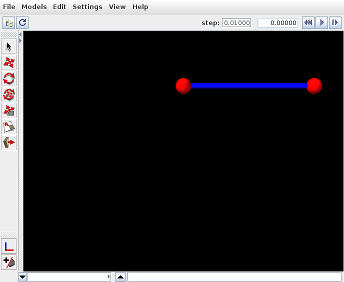
\includegraphics[]{images/ParticleSpring}
\else
 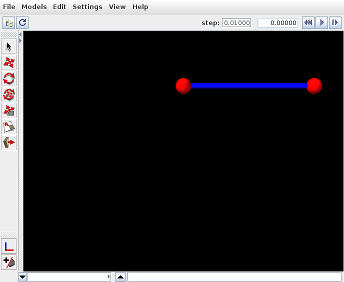
\includegraphics[width=3.75in]{images/ParticleSpring}
\fi
\end{center}
\caption{ParticleSpring model loaded into ArtiSynth.}
\label{ParticleSpring:fig}
\end{figure}

An complete application model that implements a simple particle-spring
model is given below. 
\lstset{numbers=left}
\lstinputlisting{../../src/artisynth/demos/tutorial/ParticleSpring.java}
\lstset{numbers=none}

Line 1 of the source defines the package in which the model class will
reside, in this case {\tt artisynth.demos.tutorial}. Lines 3-8 import
definitions for other classes that will be used.

The model application class is named {\tt ParticleSpring} and declared
to extend {\tt RootModel} (line 13), and the {\tt build()} method
definition begins at line 15. (A no-args constructor is also needed,
but because no other constructors are defined, the compiler creates
one automatically.)

To begin, the {\tt build()} method creates a {\tt MechModel} named
{\tt "mech"}, and then adds it to the {\tt models} list of the root model
using the {\tt addModel()} method (lines 18-19). Next, two particles,
{\tt p1} and {\tt p2}, are created, with masses equal to 2 and initial
positions at 0, 0, 0, and 1, 0, 0, respectively (lines 22-23). Then an
axial spring is created, with end points set to {\tt p1} and {\tt p2},
and assigned a linear material with a stiffness and damping of 20 and
10 (lines 24-27). Finally, after the particles and the spring are
created, they are added to the {\tt particles} and {\tt axialSprings}
lists of the {\tt MechModel} using the methods {\tt
addParticle()} and {\tt addAxialSpring()} (lines 30-32).

At this point in the code, both particles are defined to be
dynamically controlled, so that running the simulation would cause
both to fall under the {\tt MechModel}'s default gravity acceleration
of $(0, 0, -9.8)$. However, for this example, we want the first
particle to remain fixed in place, so we set it to be {\it
non-dynamic} (line 34), meaning that the physical simulation will not
update its position in response to forces (Section
\ref{DynamicVsParametric:sec}).

The remaining calls control aspects of how the model is graphicaly
rendered.  {\tt setBounds()} (line 37) increases the model's "bounding
box" so that by default it will occupy a larger part of the viewer
frustum. Both {\tt setPointRenderProps()} and {\tt
setLineRenderProps()} are convenience methods defined by the class
(lines 44-48 and 50-54) to set render properties for points and
springs, respectively. Points are set to be rendered as red spheres
with a radius of 0.06, while springs are set to be rendered as blue
cylinders with a radius of 0.02. More details about setting render
properties are given in Section \ref{RenderProperties:sec}.

To run this example in ArtiSynth, select {\sf All demos > tutorial >
ParticleSpring} from the {\sf Models} menu. The model should load and
initially appear as in Figure \ref{ParticleSpring:fig}.  Running
the model (Section \ref{LoadingAndRunning:sec}) will
cause the second particle to fall and swing about under gravity.

\subsubsection{Dynamic, parameteric, and attached components}
\label{DynamicVsParametric:sec}

By default, a dynamic component is advanced through time in response
to the forces applied to it. However, it is also possible to set a
dynamic component's {\tt dynamic} property to {\tt false}, so that it
does not respond to force inputs.  As shown in the example above, this
can be done using the method
{\tt setDynamic()}:
%
\begin{verbatim}
  comp.setDynamic (false);
\end{verbatim}
%
The method
\javamethod*[artisynth.core.mechmodels.DynamicComponent]{isDynamic()}
can be used to query the {\tt dynamic} property.

Dynamic components can also be {\it attached} to other dynamic
components (as mentioned in Section \ref{PhysicsSimulation:sec}) so
that their positions and velocities are controlled by the {\it master}
components that they are attached to.  To attach a dynamic component,
one creates an {\tt AttachmentComponent} specifying the attachment
connection and adds it to the {\tt MechModel}, as described in Section
\ref{Attachments:sec}.  The method
\javamethod*[artisynth.core.mechmodels.DynamicComponent]{isAttached()}
can be used to determine if a component is attached, and if it is,
\javamethod*[artisynth.core.mechmodels.DynamicComponent]{getAttachment()}
can be used to find the corresponding {\tt AttachmentComponent}.

Overall, a dynamic component can be in one of three states:

\begin{description}

\item[active]\mbox{}

Component is dynamic and unattached. The method
\javamethod*[artisynth.core.mechmodels.DynamicComponent]{isActive()}
returns {\tt true}. The component will move in response to forces.

\item[parametric]\mbox{}

Component is not dynamic, and is unattached. 
The method
\javamethod*[artisynth.core.mechmodels.DynamicComponent]{isParametric()}
returns {\tt true}.
The component will either remain
fixed, or will move around in response to external inputs specifying
the component's position and/or velocity. One way to supply such
inputs is to use controllers or input probes, as described in
Section \ref{SimulationControl:sec}.

\item[attached]\mbox{}

Component is attached. The method
\javamethod*[artisynth.core.mechmodels.DynamicComponent]{isAttached()}
returns {\tt true}. The component will move so as to follow the other
master component(s) to which it is attached.

\end{description}

\subsubsection{Custom axial materials}

Application authors may create their
own axial materials by subclassing 
\javaclass[artisynth.core.materials]{AxialMaterial}
and overriding the functions
%
\begin{lstlisting}[]
  double computeF (l, ldot, l0, excitation);
  double computeDFdl (l, ldot, l0, excitation);
  double computeDFdldot (l, ldot, l0, excitation);
  boolean isDFdldotZero ();
\end{lstlisting}
%
where {\tt excitation} is an additional {\it excitation} signal $a$, which
is used to implement active springs and which in particular is used to
implement axial muscles (Section \ref{PointToPointMuscles:sec}), for
which $a$ is usually in the range $[0, 1]$.

The first three methods should return the values of 
%
\begin{equation}
f (l, \dot l, a), \quad
\frac{\partial f(l, \dot l, a)}{\partial l}, \quad \text{and} \quad
\frac{\partial f(l, \dot l, a)}{\partial \dot l},
\end{equation}
%
respectively, while the last method should return {\tt true} if
$\partial f(l, \dot l, a) / \partial \dot l \equiv 0$; i.e., if it is
always equals to 0.

\subsubsection{Damping parameters}

Mechanical models usually contain damping forces in addition to
spring-type restorative forces. Damping generates forces that reduce
dynamic component velocities, and is usually the major source of
energy dissipation in the model. Damping forces can be generated by
the spring components themselves, as described above.

A general damping can be set for all particles by setting the
{\tt MechModel}'s {\tt pointDamping} property. This causes
a force
%
\begin{equation}
\f_i = -d_p \v_i
\end{equation}
%
to be applied to all particles, where $d_p$ is the value of the {\tt
pointDamping} and $\v_i$ is the particle's velocity.

{\tt pointDamping} can be set and queried using the {\tt MechModel}
methods
%
\begin{lstlisting}
  setPointDamping (double d);
  double getPointDamping();
\end{lstlisting}
%

\begin{sideblock}
In general, whenever a component has a property {\tt propX}, that
property can be set and queried in code using methods of the form
\begin{verbatim}
  setPropX (T d);
  T getPropX();
\end{verbatim}
where {\tt T} is the type associated with the property.
\end{sideblock}

{\tt pointDamping} can also be set for particles individualy.  This
property is {\it inherited} (Section
\ref{CompositeInheritableProperties:sec}), so that if not set
explicitly, it inherits the nearest explicitly set value in an
ancestor component.

\subsection{Rigid bodies}

Rigid bodies are implemented in ArtiSynth by the class
\javaclass[artisynth.core.mechmodels]{RigidBody}, which is a dynamic
component containing a six-dimensional position and orientation state,
a corresponding velocity state, an inertia, and an optional surface
mesh.

A rigid body is associated with its own 3D spatial coordinate frame,
and is a subclass of the more general
\javaclass[artisynth.core.mechmodels]{Frame} component.
The combined position and orientation of this frame with respect to
world coordinates defines the body's {\it pose}, and the associated 6
degrees of freedom decribe its "position" state.

\subsubsection{Frame markers}
\label{FrameMarkers:sec}

\begin{figure}[t]
\begin{center}
 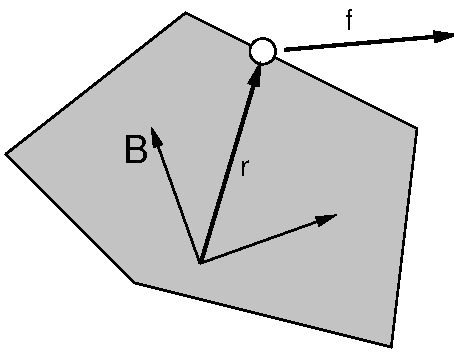
\includegraphics[width=2.5in]{images/frameMarker}
\end{center}
\caption{A force $\f$ applied to a frame marker attached to a rigid
body. The marker is located at the point $\r$ with respect to the body
coordinate frame B.}
\label{frameMarker:fig}
\end{figure}

ArtiSynth makes extensive use of {\it markers}, which are (massless)
points attached to dynamic components in the model. Markers are used
for graphical display, implementing attachments, and transmiting
forces back onto the underlying dynamic components.

A {\it frame marker} is a marker that can be attached to a
\javaclass[artisynth.core.mechmodels]{Frame}, and most commonly to a
\javaclass[artisynth.core.mechmodels]{RigidBody} (Figure
\ref{frameMarker:fig}). They are frequently used to provide the
anchor points for attaching springs and, more generally, applying
forces to the body.

Frame markers are implemented by the class
\javaclass[artisynth.core.mechmodels]{FrameMarker}, which
is a subclass of
\javaclass[artisynth.core.mechmodels]{Point}.
The methods
%
\begin{lstlisting}
  Point3d getLocation();
  void setLocation (Point3d r);
\end{lstlisting}
%
get and set the marker's location $\r$ with respect to the frame's
coordinate system. When a 3D force $\f$ is applied to the marker, it
generates a spatial force $\hat\f$ (Section
\ref{SpatialVelocitiesAndForces:sec}) on the frame given by
%
\begin{equation}
\hat\f = \matl \f \\ \r \times \f \matr.
\end{equation}
%

\begin{figure}[h]
\begin{center}
\iflatexml
 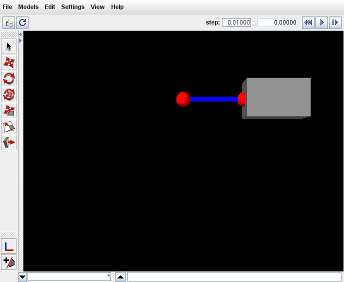
\includegraphics[]{images/RigidBodySpring}
\else
 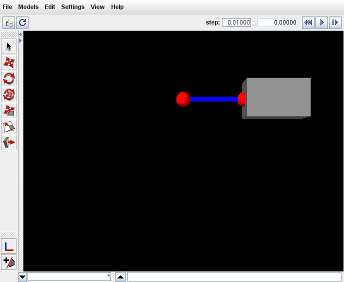
\includegraphics[width=3.75in]{images/RigidBodySpring}
\fi
\end{center}
\caption{RigidBodySpring model loaded into ArtiSynth.}
\label{RigidBodySpring:fig}
\end{figure}

\subsubsection{Example: A simple rigid body-spring model}
\label{RigidBodySpringExample:sec}

A simple rigid body-spring model is defined in
%
\begin{verbatim}
  artisynth.demos.tutorial.RigidBodySpring
\end{verbatim}
%
This differs from ParticleSpring only in the {\tt build()} method,
which is listed below:
\lstset{numbers=left}
\begin{lstlisting}
   public void build (String[] args) {

      // create MechModel and add to RootModel
      MechModel mech = new MechModel ("mech");
      addModel (mech);

      // create the components
      Particle p1 = new Particle ("p1", /*mass=*/2, /*x,y,z=*/0, 0, 0);
      // create box and set it's pose (position/orientation):
      RigidBody box =
         RigidBody.createBox ("box", /*wx,wy,wz=*/0.5, 0.3, 0.3, /*density=*/20);
      box.setPose (new RigidTransform3d (/*x,y,z=*/0.75, 0, 0));
      // create marker point and connect it to the box:
      FrameMarker mkr = new FrameMarker (/*x,y,z=*/-0.25, 0, 0);
      mkr.setFrame (box);

      AxialSpring spring = new AxialSpring ("spr", /*restLength=*/0);
      spring.setPoints (p1, mkr);
      spring.setMaterial (
         new LinearAxialMaterial (/*stiffness=*/20, /*damping=*/10));

      // add components to the mech model
      mech.addParticle (p1);
      mech.addRigidBody (box);
      mech.addFrameMarker (mkr);
      mech.addAxialSpring (spring);

      p1.setDynamic (false);               // first particle set to be fixed

      // increase model bounding box for the viewer
      mech.setBounds (/*min=*/-1, 0, -1, /*max=*/1, 0, 0);  
      // set render properties for the components
      setPointRenderProps (p1);
      setPointRenderProps (mkr);
      setLineRenderProps (spring);
   }
\end{lstlisting}
\lstset{numbers=none} 
The differences from {\tt ParticleSpring} begin
at line 9. Instead of creating a second particle, a rigid body is
created using the factory method
\javamethod*[artisynth.core.mechmodels]{RigidBody.createBox()}, which
takes x, y, z widths and a (uniform) density and creates a box-shaped
rigid body complete with surface mesh and appropriate mass and
inertia. As the box is initially centered at the origin, moving it
elsewhere requires setting the body's pose, which is done using {\tt
setPose()}. The {\tt RigidTransform3d} passed to {\tt setPose()} is
created using a three-argument constructor that generates a
translation-only transform.  Next, starting at line 14, a {\tt
FrameMarker} is created for a location $(-0.25, 0, 0)^T$ relative to the
rigid body, and attached to the body using its {\tt setFrame()}
method.

The remainder of {\tt build()} is the same as for {\tt ParticleSpring},
except that the spring is attached to the frame marker instead of a
second particle.

To run this example in ArtiSynth, select {\sf All demos > tutorial >
RigidBodySpring} from the {\sf Models} menu. The model should load and
initially appear as in Figure \ref{RigidBodySpring:fig}.  Running the
model (Section \ref{LoadingAndRunning:sec}) will cause the rigid body
to fall and swing about under gravity.

\subsubsection{Creating rigid bodies}

As illustrated above, rigid bodies can be created using factory
methods supplied by \javaclass[artisynth.core.mechmodels]{RigidBody}.
Some of these include:
%
\begin{lstlisting}
  createBox (name, widthx, widthy, widthz, density);
  createCylinder (name, radius, height, density, nsides);
  createSphere (name, radius, density, nslices);
  createEllipsoid (name, radx, rady, radz, density, nslices);
\end{lstlisting}
%
The bodies do not need to be named; if no name is desired, then {\tt
name} and can be specified as {\tt null}.

In addition, there are also
factory methods for creating a rigid body directly from a mesh:
%
\begin{lstlisting}
  createFromMesh (name, mesh, density, scale);
  createFromMesh (name, meshFileName, density, scale);
\end{lstlisting}
%
These take either a polygonal mesh (Section \ref{Meshes:sec}), or a
file name from which a mesh is read, and use it as the body's surface
mesh and then compute the mass and inertia properties from the specified
(uniform) density.

Alternatively, one can create a rigid body directly from a
constructor, and then set the mesh and inertia properties explicitly:
%
\begin{lstlisting}[]
  PolygonalMesh femurMesh;
  SpatialInertia inertia;

  ... initialize mesh and inertia appropriately ...

  RigidBody body = new RigidBody ("femur");
  body.setMesh (femurMesh);
  body.setInertia (inertia);
\end{lstlisting}
%

\subsubsection{Pose and velocity}

A body's pose can be set and
queried using the methods
%
\begin{lstlisting}[]
  setPose (RigidTransform3d T);   // sets the pose to T
  getPose (RigidTransform3d T);   // gets the current pose in T
  RigidTransform3d getPose();     // returns the current pose (read-only)
\end{lstlisting}
%
These use a \javaclass[maspack.matrix]{RigidTransform3d} (Section
\ref{RigidTransform3d:sec}) to describe the pose. Body poses are
described in world coordinates and specify the transform from body to
world coordinates. In particular, the pose for a body A specifies
the rigid transform $\T_{AW}$.

Rigid bodies also expose the translational and rotational components of
their pose via the properties {\tt position} and {\tt orientation},
which can be queried and set independently using the methods
%
\begin{lstlisting}[]
  setPosition (Point3d p);       // sets the position to p
  getPosition (Point3d p);       // gets the current position in p
  Point3d getPosition();         // returns the current position (read-only)

  setOrientation (AxisAngle a);  // sets the orientation to a
  getOrientation (AxisAngle a);  // gets the current orientation in a
  AxisAngle getOrientation();    // returns the current orientation (read-only)
\end{lstlisting}
%

The velocity of a rigid body is described using a
\javaclass[maspack.spatialmotion]{Twist} (Section
\ref{SpatialVectors:sec}), which contains both the translational and
rotational velocities. The following methods
set and query the spatial velocity as described with respect to world
coordinates:
%
\begin{lstlisting}[]
  setVelocity (Twist v);         // sets the spatial velocity to v
  getVelocity (Twist v);         // gets the current spatial velocity in v
  Twist getVelocity();           // returns current spatial velocity (read-only)
\end{lstlisting}
%

During simulation, unless a rigid body has been set to be {\it
parametric} (Section \ref{DynamicVsParametric:sec}), its pose and
velocity are updated in response to forces, so setting the pose or
velocity generally makes sense only for setting initial conditions.
On the other hand, if a rigid body is parametric, then it is possible
to control its pose during the simulation, but in that case it is
better to set its {\it target pose} and/or {\it target velocity}, as
described in Section \ref{ControllerImplementation:sec}.

\subsubsection{Inertia and meshes}

The "mass" of a rigid body is described by its spatial inertia
(Section \ref{SpatialInertia:sec}), implemented by a
\javaclass[maspack.spatialmotion]{SpatialInertia} object, which
specifies its mass, center of mass, and rotational inertia with
respect to the center of mass.

Most rigid bodies are also associated with a polygonal surface mesh,
which can be set and queried using the methods
%
\begin{lstlisting}
  setMesh (PolygonalMesh mesh);
  setMesh (PolygonalMesh mesh, String meshFileName);
  PolygonalMesh getMesh();
\end{lstlisting}
%
The second method takes an optional {\tt fileName} argument that can
be set to the name of a file from which the mesh was read. Then if the
model itself is saved to a file, the model file will specify the mesh
using the file name (instead of explicit vertex and face information),
which can reduce the model file size considerably.

The inertia of a rigid body can be explicitly set using a variety
of methods including
%
\begin{lstlisting}
  setInertia (M)                    // SpatialInertia
  setInertia (mass, Jxx, Jyy, Jzz); // mass and diagonal rotational inertia
  setInertia (mass, J);             // mass and full rotational inertia
  setInertia (mass, J, com);        // mass, rotational inertia, center-of-mass
\end{lstlisting}
%
and can be queried using 
%
\begin{lstlisting}
  getInertia (M);                   // get SpatialInertia in M
  getInertia ();                    // return read-only SpatialInertia
\end{lstlisting}
%

In practice, it is often more convenient to simply specify a mass or a
density, and then use the volume defined by the surface mesh to
compute the remaining inertial values. How a rigid body's inertia is
computed is determined by its {\tt inertiaMethod} property, which can
be one

\begin{description}

\item[Density]\mbox{}

Inertia is computed from density;

\item[Mass]\mbox{}

Inertia is computed from mass;

\item[Explicit]

Inertia is set explicitly.

\end{description}

This property can be set and queried using
%
\begin{lstlisting}
  setInertiaMethod (InertiaMethod method);
  InertiaMethod getInertiaMethod();
\end{lstlisting}
%
and it's default value is {\tt Density}. Explicitly setting the
inertia using one of the above {\tt setInertia()} methods will cause
the value to change to {\tt Explicit}. The method
%
\begin{lstlisting}
  setInertiaFromDensity (density); 
\end{lstlisting}
%
will (re)compute the inertia using the mesh and a density value
and set {\tt inertiaMethod} to {\tt Density}, and
the method
%
\begin{lstlisting}
  setInertiaFromMass (mass); 
\end{lstlisting}
%
will (re)compute the inertia using the mesh and mass value
and set {\tt inertiaMethod} to {\tt Mass}.

Finally, the (assumed uniform) density of the body can be queried
using
%
\begin{lstlisting}
   getDensity();
\end{lstlisting}
%

\subsubsection{Damping parameters}
\label{RigidBodyDamping:sec}

As with particles, it is possible to set damping parameters for rigid
bodies. 

{\tt MechModel} provides two properties, {\tt frameDamping} and {\tt
rotaryDamping}, which generate a spatial force centered on each rigid
body's coordinate frame
%
\begin{equation}
\hat\f_i = \matl -d_f \v_i \\ -d_r \Bom_i \matr,
\end{equation}
%
where $d_f$ and $d_r$ are the {\tt frameDamping} and {\tt
rotaryDamping} values, and $\v_i$ and $\Bom_i$ are the translational
and angular velocity of the body's coordinate frame.
The damping parameters can be set and queried using the {\tt MechModel}
methods
%
\begin{lstlisting}
  setFrameDamping (double df);
  setRotaryDamping (double dr);
  double getFrameDamping();
  double getRotaryDamping();
\end{lstlisting}
%

Frame and rotatary damping can also be set for individual bodies using
their own (inherited) {\tt frameDamping} and {\tt rotaryDamping}
properties.

\subsection{Joints and connectors}

In a typical mechanical model, many of the rigid bodies are
interconnected, either using spring-type components that exert binding
forces on the bodies, or through joint-type connectors that enforce
the connection using hard constraints.

\subsubsection{Joints and coordinate frames}

Consider two bodies A and B. The pose of body B with respect to body A
can be described by the 6 DOF rigid transform $\T_{BA}$.  If bodies A
and B are unconnected, that $\T_{BA}$ may assume any possible value
and has a full six degrees of freedom. A {\it joint} between A and B
restricts the set of poses that are possible between the two bodies
and reduces the degrees of freedom available to $\T_{BA}$.  For
simplicity, joints have their own coordinate frames for describing
their constraining actions, and then these frames are related to the
frames of the associated bodies by auxiliary transformations.

\begin{figure}[h]
\begin{center}
 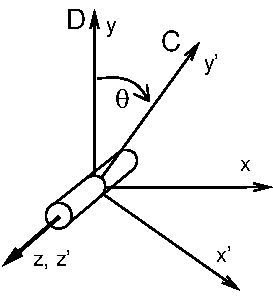
\includegraphics[width=2.5in]{images/jointExample}
\end{center}
\caption{Coordinate frames D and C for a revolute joint.}
\label{jointExample:fig}
\end{figure}

Each joint is associated with two coordinate frames C and D which move
with respect to each other as the joint moves. The allowed joint
motions therefore correspond to the allowed values of the {\it joint transform}
$\T_{CD}$.  D is the {\it base} frame and C is the {\it constraint}
frame. For a revolute joint (Figure \ref{jointExample:fig}), C can
move with respect to D by rotating about the z axis. Other motions are
prohbited. $\T_{CD}$ should therefore alway have the form
%
\begin{equation}
\T_{CD} = \matl
\cos(\theta) & -sin(\theta) & 0 \\
\sin(\theta) &  cos(\theta) & 0 \\
0 & 0 & 1\\
\matr
\end{equation}
%
where $\theta$ is the angle of joint rotation and is known as the {\it
joint parameter}. Other joints have different parameterizations, with
the number of parameters equaling the number of degrees of freedom
available to the joint. When $\T_{CD} = \I$ (where $\I$ is the
identity transform), the parameters are all (usually) equal to zero,
and the joint is said to be in the {\it zero state}.

\begin{figure}[h]
\begin{center}
 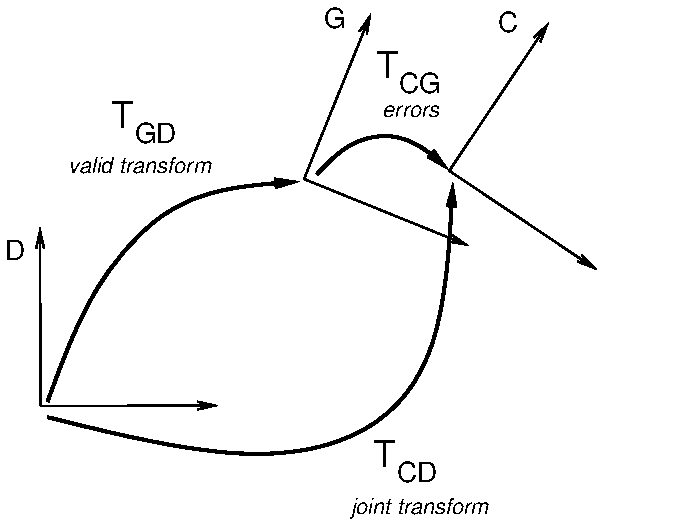
\includegraphics[width=2.5in]{images/jointFrames}
\end{center}
\caption{2D schematric showing the joint frames D and C, along with
the intermediate frame G that accounts for numeric error
and complaint motion.}
\label{jointFrames:fig}
\end{figure}

In practice, due to numerical errors and/or compliance in the joint
(Section \ref{JointCompliance:sec}), the joint transform $\T_{CD}$ may
sometimes deviate from the allowed set of values dictated by the joint
type. In ArtiSynth, this is accounted for by introducing an additional
{\it constraint} frame G between D and C (Figure \ref{jointFrames:fig}).
G is computed to be the nearest frame to C that lies exactly 
in the joint constraint space. $\T_{GD}$ is therefore a
valid transform for the joint, $\T_{GC}$ accomodates the error,
and the whole joint transform is given by the composition
%
\begin{equation}
\T_{CD} = \T_{GD} \; \T_{CG}.
\end{equation}
%
If there is no compliance or joint error, then frames G and C are the
same, $\T_{CG} = \I$, and $\T_{CD} = \T_{GD}$.

In general, each joint is attached to two rigid bodies A and B, with
frame C being fixed to body A and frame D being fixed to body B. The
restrictions of the joint transform $\T_{CD}$ therefore restrict the
relative poses of A and B.

\begin{figure}[h]
\begin{center}
 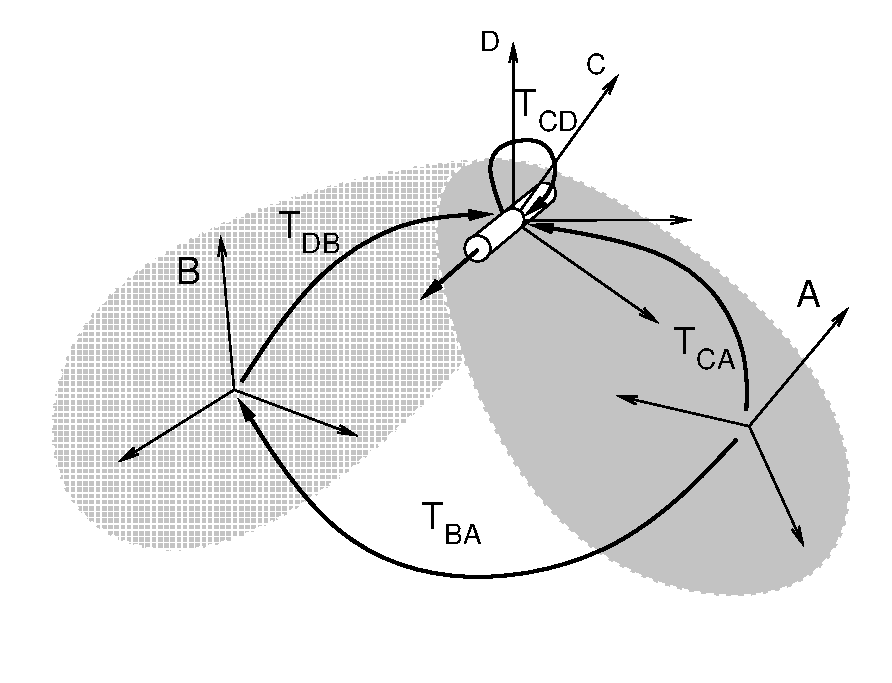
\includegraphics[width=3.74in]{images/jointBodyFrames}
\end{center}
\caption{Tranforms connecting joint coordinate frames C and D with
rigid bodies A and B.}
\label{jointBodyFrames:fig}
\end{figure}

Except in special cases, the joint coordinate frames C and D are not
coincident with the body frames A and B.  Instead, they are located
relative to A and B by the transforms $\T_{CA}$ and $\T_{DB}$,
respectively (Figure \ref{jointBodyFrames:fig}). 
Since $\T_{CA}$ and $\T_{DB}$ are both fixed, the pose
of B relative to A can be determined from
the joint transform $\T_{CD}$:
%
\begin{equation}
\T_{BA} = \T_{CA} \, \T_{CD}^{-1} \, \T_{DB}^{-1}.
\label{jointPose:eqn}
\end{equation}
%
(See Section \ref{RigidTransforms:sec} for a discussion of determining
transforms between related coordinate frames).

\subsubsection{Creating Joints}
\label{CreatingJoints:sec}

Joint components in ArtiSynth are implemented by subclasses of
\javaclass[artisynth.core.mechmodels]{RigidBodyConnector}.  Some of
the commonly used ones are described in Section
\ref{CommonJoints:sec}.

An application creates a joint by constructing it and adding it to a
{\tt MechModel}. Most joints generally have a constructor of the form
%
\begin{lstlisting}
  JointType (bodyA, bodyB, XDW);
\end{lstlisting}
%
which specifies the rigid bodies A and B which the joint connects,
along with the transform $\T_{DW}$ giving the pose of the joint base
frame D in world coordinates. Then constructor then assumes that the
joint is in the zero state, so that $\T_{CD} = \I$ and C and D are
the same, and then computes
$\T_{CA}$ and $\T_{DB}$ from
%
\begin{align}
\T_{CA} & = \T_{AW}^{-1} \; \T_{DW} \\
\T_{DB} & = \T_{BW}^{-1} \; \T_{DW}
\end{align}
%
where $\T_{AW}$ and $\T_{BW}$ are the poses of A and B.
The same body and transform settings can be made on an existing
joint using the method
\javamethodAlt{%
artisynth.core.mechmodels.RigidBodyConnector.setBodies(,,)}
{setBodies(bodyA, bodyB, XDW)}.

Alternatively, if we prefer to specify $\T_{CA}$ or $\T_{BA}$, then we
can determine $\T_{DW}$ from $\T_{AW}$ or $\T_{BW}$ using
%
\begin{align}
\T_{DW} & = \T_{AW} \; \T_{CA} \\
\T_{DW} & = \T_{BW} \; \T_{DB}.
\end{align}
%
For example, if we know $\T_{CA}$, this can be accomplished using
the following code fragment:
%
\begin{lstlisting}
   RigidBody bodyA, bodyB;
   RigidTransform3d TCA;

   ... initialize bodyA, bodyB, and TCA ...
   
   RigidTransform3d TDW = new RigidTransform3d();
   TDW.mul (bodyA.getPose(), TCA);  // bodyA.getPose() returns TAW
   RevoluteJoint joint = new RevoluteJoint (bodyA, bodyB, TDW);
\end{lstlisting}
%

Another method,
\javamethodAlt{artisynth.core.mechmodels.RigidBodyConnector.setBodies(,,,)}
{setBodies(bodyA, XCA, bodyB, XDB)}, allows us to set both values of
$\T_{CA}$ or $\T_{BA}$ explicity. This is useful if the joint
transform $\T_{CD}$ is known to be some value {\it other} than the
identity, in which case $\T_{CA}$ or $\T_{BA}$ can be computed
from (\ref{jointPose:eqn}), where $\T_{BA}$ is given by
%
\begin{equation}
\T_{BA} = \T_{AW}^{-1} \; \T_{BW}.
\end{equation}
%
For instance, if we know $\T_{CA}$ and the joint transform $\T_{CD}$,
then we can compute $\T_{DB}$
from
%
\begin{equation}
\T_{DB} = \T_{BA}^{-1} \, \T_{CA} \, \T_{CD}^{-1} = 
\T_{BW}^{-1}  \, T_{AW} \, \T_{CA} \, \T_{CD}^{-1}
\end{equation}
%
and set up the joint as follows:
%
\begin{lstlisting}
   RigidBody bodyA, bodyB;
   RigidTransform3d TCA, TCD;

   ... initialize bodyA, bodyB, TCA, TCD ...
   
   RigidTransform3d TBD = new RigidTransform3d();
   TDB.mulInverseLeft (bodyB.getPose(), bodyA.getPose());
   TDB.mul (TCA);
   TDB.mulInverse (TCD);
   RevoluteJoint joint = new RevoluteJoint ();
   joint.setBodies (bodyA, TCA, bodyB, TDB);
\end{lstlisting}
%

Some joint implementations provide the ability to explictly set the
joint parameter(s) after it has been created and added to the {\tt
MechModel}, making it easy to "move" the joint to a specific
configuration. For example, {\tt RevoluteJoint} provides the method
\javamethod*[artisynth.core.mechmodels.RevoluteJoint]{setTheta()}.
This causes the transform $\T_{CD}$ to be explicity set to the value
implied by the joint parameters, and the pose of either body A or B is
changed to accommodate this. Whether body A or B is moved depends on
which one is the least connected to ground, and other bodies that have
joint connections to the moved body are moved as well.

If desired, joints can be connected to only a single rigid body. In
this case, the second body B is simply assumed to be "ground", and the
coordinate frame that would be associated with body B is instead taken
to be the world coordinate frame W. The corresponding calls
to the joint constructor or {\tt setBodies()} take the
form
%
\begin{lstlisting}
  joint = new JointType (bodyA, null, XDW);
  joint.setBodies (bodyA, null, XDW);
\end{lstlisting}
%

\subsubsection{Example:  A simple revolute joint}
\label{RigidBodyJoint:sec}

\begin{figure}[h]
\begin{center}
\iflatexml
 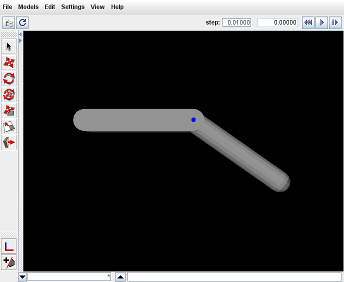
\includegraphics[]{images/RigidBodyJoint}
\else
 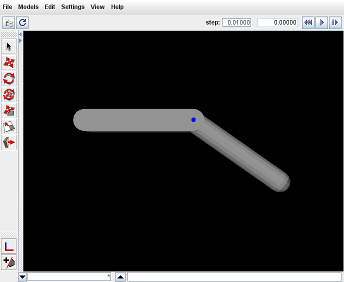
\includegraphics[width=3.75in]{images/RigidBodyJoint}
\fi
\end{center}
\caption{RigidBodyJoint model loaded into ArtiSynth.}
\label{RigidBodyJoint:fig}
\end{figure}

A simple model showing two rigid bodies connected by
a joint is defined in
%
\begin{verbatim}
  artisynth.demos.tutorial.RigidBodyJoint
\end{verbatim}
%

The build method for this model is given below:
\lstset{numbers=left}
\begin{lstlisting}
   public void build (String[] args) {

      // create MechModel and add to RootModel
      mech = new MechModel ("mech");
      mech.setGravity (0, 0, -98);
      mech.setFrameDamping (1.0);
      mech.setRotaryDamping (4.0);
      addModel (mech);

      PolygonalMesh mesh;  // bodies will be defined using a mesh

      // create first body and set its pose
      mesh = MeshFactory.createRoundedBox (lenx1, leny1, lenz1, /*nslices=*/8);
      RigidTransform3d TMB = 
         new RigidTransform3d (0, 0, 0, /*axisAng=*/1, 1, 1, 2*Math.PI/3);
      mesh.transform (TMB);
      bodyB = RigidBody.createFromMesh ("bodyB", mesh, /*density=*/0.2, 1.0);
      bodyB.setPose (new RigidTransform3d (0, 0, 1.5*lenx1, 1, 0, 0, Math.PI/2));
      bodyB.setDynamic (false);

      // create second body and set its pose
      mesh = MeshFactory.createRoundedCylinder (
         leny2/2, lenx2, /*nslices=*/16, /*nsegs=*/1, /*flatBottom=*/false);
      mesh.transform (TMB);
      bodyA = RigidBody.createFromMesh ("bodyA", mesh, 0.2, 1.0);
      bodyA.setPose (new RigidTransform3d (
                        (lenx1+lenx2)/2, 0, 1.5*lenx1, 1, 0, 0, Math.PI/2));

      // create the joint      
      RigidTransform3d TDW = 
         new RigidTransform3d (lenx1/2, 0, 1.5*lenx1, 1, 0, 0, Math.PI/2);
      RevoluteJoint joint = new RevoluteJoint (bodyA, bodyB, TDW);

      // add components to the mech model
      mech.addRigidBody (bodyB);
      mech.addRigidBody (bodyA);
      mech.addRigidBodyConnector (joint);

      joint.setTheta (35);  // set joint position

      // set render properties for components
      RenderProps.setLineRadius (joint, 0.2);
      joint.setAxisLength (4);
   }
\end{lstlisting}
\lstset{numbers=none}

A {\tt MechModel} is created as usual at line 4. However, in this
example, we also set some parameters for it:
\javamethod*[artisynth.core.mechmodels.MechModel]{setGravity()} is used to set
the gravity acceleration vector to $(0, 0, -98)^T$ instead of the
default value of $(0, 0, -9.8)^T$, and frame and rotary damping
(Section \ref{RigidBodyDamping:sec}) are set to provide dissipation.

Each of the two rigid bodies are created from a mesh and a density.
The meshes themselves are created using the factory methods
\javamethod*[maspack.geometry]{MeshFactory.createRoundedBox()} and
\javamethod*[maspack.geometry]{MeshFactory.createRoundedCylinder()}
(lines 13 and 22), and then
\javamethod*[artisynth.core.mechmodels]{RigidBody.createFromMesh()} is
used to turn these into rigid bodies with a density of 0.2 (lines 17
and 25). The pose of the two bodies is set using {\tt
RigidTransform3d} objects created with x, y, z translation and
axis-angle orientation values (lines 18 and 26).

The revolute joint is implemented using
\javaclass[artisynth.core.mechmodels]{RevoluteJoint}, which is
constructed at line 32 with the joint coordinate frame D being located
in world coordinates by {\tt TDW} 
as described in Section \ref{CreatingJoints:sec}.

Once the joint is created at added to the {\tt MechModel}, the method
\javamethod*[artisynth.core.mechmodels.RevoluteJoint]{setTheta()} is
used to explicity set the joint parameter to 35 degrees. The joint
transform $\T_{CD}$ is then set appropriately and {\tt bodyA} is moved
to accommodate this ({\tt bodyA} being chosen since it is the freeest
to move).

Finally, render properties are set starting at line 42. A revolute
joint is rendered as a line segment, using the line render properties,
with {\tt lineStyle} and {\tt lineColor} set to {\tt Cylinder} and
{\tt BLUE} by default. The cylinder radius and length are specified by
the line render property {\tt lineRadius} and the revolute joint
property {\tt axisLength}, which are set explicitly in the code.

To run this example in ArtiSynth, select {\sf All demos > tutorial >
RigidBodySpring} from the {\sf Models} menu. The model should load and
initially appear as in Figure \ref{RigidBodyJoint:fig}.  Running the
model (Section \ref{LoadingAndRunning:sec}) will cause {\tt bodyA} to
fall and swing under gravity.

\subsubsection{Commonly used joints}
\label{CommonJoints:sec}

\begin{figure}
\begin{center}
\begin{tabular}{cc}
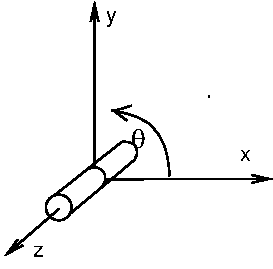
\includegraphics[width=1.75in]{images/revoluteJoint}&
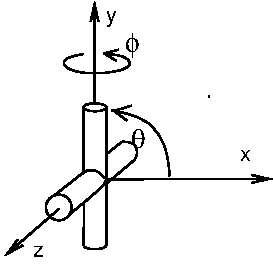
\includegraphics[width=1.75in]{images/rollPitchJoint}\\
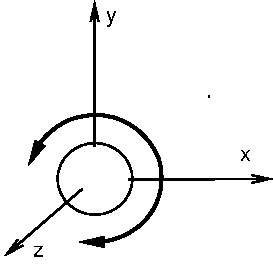
\includegraphics[width=1.75in]{images/sphericalJoint}&
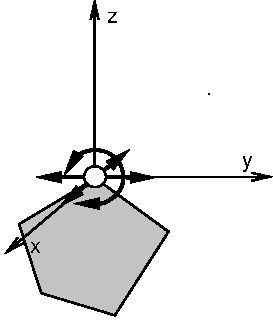
\includegraphics[width=1.75in]{images/planarConnector}\\
\end{tabular}
\end{center}
\caption{Commonly used joints. Clockwise from
top left: revolute, roll-pitch, spherical, planer connector.}
\label{CommonJoints:fig}
\end{figure}

Some of the joints commonly used by ArtiSynth are shown in Figure
\ref{CommonJoints:fig}. Each illustration shows the allowed joint
motion relative to the base coordinate frame D. Clockwise
from the top-left, these joints are:

\begin{description}

\item[Revolute joint]

A one DOF joint which allows rotation by a angle $\theta$ about
the z axis.

\item[Roll-pitch joint]

A two DOF joint, similar to the revolute joint, which allows the
rotation about z to be followed by an additional rotation $\phi$ about
the (new) y axis.

\item[Spherical joint]

A three DOF joint in which the origin remains fixed but any orientation
may be assumed.

\item[Planar connector]

A five DOF joint which connects a point on a single rigid body to a
plane in space. The point may slide freely in the x-y plane, and the
body may assume any orientation about the point.

\end{description}

\subsubsection{Joint Compliance}
\label{JointCompliance:sec}

OPTIONAL

\subsection{Frame springs}

Another way to connect two rigid bodies together is to use a {\it
frame spring}, which is a six dimensional spring that generates
restoring forces and moments between coordinate frames.

\subsubsection{Frame spring coordinate frames}

\begin{figure}[h]
\begin{center}
 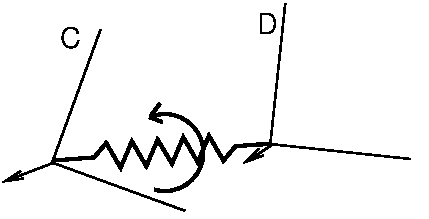
\includegraphics[width=3in]{images/frameSpring}
\end{center}
\caption{A frame spring connecting two coordinate frames D and C.}
\label{frameSpring:fig}
\end{figure}

The basic idea of a frame spring is shown in Figure
\ref{frameSpring:fig}. It generates restoring forces and moments on
two frames C and D which are a function of $\T_{DC}$ and $\hat\v_{DC}$
(the spatial velocity of frame D with respect to frame C).

Decomposing forces into stiffness and damping terms, the force
$\f_c$ and moment $\Btau_c$ acting on C can be expressed as 
%
\begin{align}
\f_C & = \f_{Ck} (\T_{DC}) + \f_{Cd} (\hat\v_{DC}) \notag \\
\Btau_C & = \Btau_{Ck} (\T_{DC}) + \Btau_{Cd} (\hat\v_{DC}).
\label{ftauC:eqn}
\end{align}
%
The forces acting on D are equal and opposite, so that
%
\begin{align}
\f_D & = - \f_C, \notag \\
\Btau_D & = - \Btau_C.
\label{ftau2:eqn}
\end{align}
%

\begin{figure}[h]
\begin{center}
 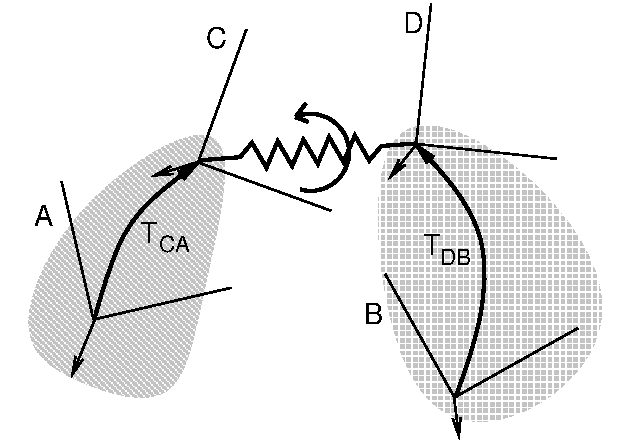
\includegraphics[width=3in]{images/frameSpringBodies}
\end{center}
\caption{A frame spring connecting two rigid bodies A and B.}
\label{frameSpringBodies:fig}
\end{figure}

If frames C and D are attached to a pair of rigid bodies A and B, then
a frame spring can be used to connect them in a manner analogous to a
joint. As with joints, C and D generally do not coincide with the body
frames, and are instead offset from them by fixed transforms $\T_{CA}$
and $\T_{DB}$ (Figure \ref{frameSpringBodies:fig}).

\subsubsection{Frame materials}

The restoring forces (\ref{ftauC:eqn}) generated in a frame spring
depends on the {\it frame material} associated with the spring. Frame
materials are defined in the package {\tt artisynth.core.materials},
and are subclassed from
\javaclass[artisynth.core.materials]{FrameMaterial}.
The most basic type of material is a 
\javaclass[artisynth.core.materials]{LinearFrameMaterial},
in which the restoring forces are determined from
%
\begin{align*}
\f_C & = 
\K_{f} \, \x_{DC} + \D_{f} \, \v_{DC} \\
\Btau_C & = 
\K_{\tau} \, \hat\Bthe_{DC} + \D_{\tau} \, \Bom_{DC}
\label{flinear:eqn}
\end{align*}
%
where $\hat\Bthe_{DC}$ gives the small angle approximation of the
rotational components of $\X_{DC}$ with respect to the $x$, $y$, and
$z$ axes, and
%
\begin{gather*}
\K_{t} \equiv 
\matl k_{tx} & 0 & 0 \\ 0 & k_{ty} & 0 \\ 0 & 0 & k_{tz} \matr, \;
\D_{t} \equiv 
\matl d_{tx} & 0 & 0 \\ 0 & d_{ty} & 0 \\ 0 & 0 & d_{tz} \matr, \;\\
\K_{r} \equiv
\matl k_{r x} & 0 & 0 \\ 0 & k_{r y} & 0 \\ 0 & 0 & k_{r z} \matr, \;
\D_{r} \equiv
\matl d_{r x} & 0 & 0 \\ 0 & d_{r y} & 0 \\ 0 & 0 & d_{r z} \matr.
\end{gather*}
%
are the stiffness and damping matrices. The stiffness and damping
values $\k_t$, $\k_r$, $\d_t$, and $\d_ru$ are exposed as the
{\tt stiffness}, {\tt rotaryStiffness}, {\tt damping}, and {\tt
rotaryDamping} properties of the material. Each of these is a 3
dimensional vector giving stiffness or damping values along or about a
particular axis. Specifying different values for different axes will
result in an anisotropic behavior.

Other frame materials offering nonlinear behaviour may be defined in
{\tt artisynth.core.materials}.

\subsubsection{Creating frame springs}
\label{CreatingFrameSprings:sec}

Frame springs are implemented by the class
\javaclass[artisynth.core.mechmodels]{FrameSpring}.  Creating a frame
spring generally involves instantiating this class, and then setting
the material, the bodies A and B, and the transforms $\T_{CA}$ and
$\T_{DB}$.

A typical construction sequence might look like this:
%
\begin{lstlisting}
  FrameSpring spring = new FrameSpring ("springA");
  spring.setMaterial (new LinearFrameMaterial (kt, kr, dt, dr));
  spring.setFrames (bodyA, bodyB, TDW);
\end{lstlisting}
%
The material is set using
\javamethod*[artisynth.core.mechmodels.FrameSpring]{setMaterial()}.
The example above uses a {\tt LinearFrameMaterial}, created with a
constructor that sets $\k_t$, $\k_r$, $\d_t$, and $\d_ru$ to uniform
isotropic values specified by {\tt kt}, {\tt kr}, {\tt dt}, and {\tt
dr}. 

The bodies and transforms can be set in the same manner as for joints
(Section \ref{CreatingJoints:sec}), with the methods
\javamethodAlt{artisynth.core.mechmodels.FrameSpring.setFrames(Frame,Frame,RigidTransform3d)}{setFrames(bodyA,bodyB,TDW)}
and
\javamethodAlt{artisynth.core.mechmodels.FrameSpring.setFrames(Frame,RigidTransform3d,Frame,RigidTransform3d)}{setFrames(bodyA,TCA,bodyB,TDB)}
assuming the role of {\tt setBodies(bodyA,bodyB,TDW)} and
{\tt setBodies(bodyA,TCA,bodyB,TDB)} (rigid bodies are instances of the
more general {\tt Frame} class). The former takes D specified in
worlds coordinates and computes $\T_{CA}$ and $\T_{DB}$ assuming that
there is no initial spring displacement (i.e., that $\T_{DC} = \I$),
while the latter allows $\T_{CA}$ and $\T_{DB}$ to be specified
explicitly.

Frame springs and joints are often placed together, using the same
transforms $\T_{CA}$ and $\T_{CB}$, with the spring providing
restoring forces tp help keep the joint within presribed bounds.

As with joints, a frame spring can be connected to only a single body,
by specifying {\tt frameB} as {\tt null}. Frame B is then taken to be
the world coordinate frame W.

\subsubsection{Example: Two bodies connected by a frame spring}

\begin{figure}[h]
\begin{center}
\iflatexml
 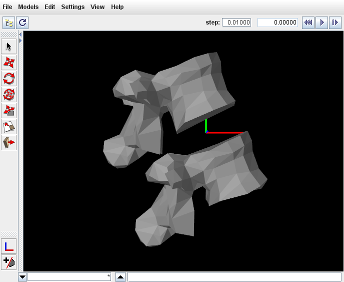
\includegraphics[]{images/LumbarFrameSpring}
\else
 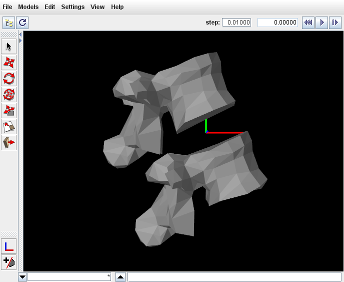
\includegraphics[width=3.75in]{images/LumbarFrameSpring}
\fi
\end{center}
\caption{LumbarFrameSpring model loaded into ArtiSynth.}
\label{LumbarFrameSpring:fig}
\end{figure}

A simple model showing two simplified lumbar vertebrae, modeled as
rigid bodies and connected by a frame spring, is defined in
%
\begin{verbatim}
  artisynth.demos.tutorial.LumbarFrameSpring
\end{verbatim}
%
and most of the code for this is shown here:
%
\lstset{numbers=left}
\begin{lstlisting}
   // path from which meshes will be read
   private String geometryDir = ArtisynthPath.getSrcRelativePath (
      LumbarFrameSpring.class, "../mech/geometry/");

   // create and add a rigid body from a mesh
   public RigidBody addBone (MechModel mech, String name) throws IOException {
      PolygonalMesh mesh = new PolygonalMesh (new File (geometryDir+name+".obj"));
      RigidBody rb = RigidBody.createFromMesh (name, mesh, density, /*scale=*/1);
      mech.addRigidBody (rb);
      return rb;
   }

   public void build (String[] args) throws IOException {

      // create mech model and set it's properties
      MechModel mech = new MechModel ("mech");
      mech.setGravity (0, 0, -1.0);
      mech.setFrameDamping (0.10);
      mech.setRotaryDamping (0.001);
      addModel (mech);

      // create two rigid bodies and second one to be fixed
      RigidBody lumbar1 = addBone (mech, "lumbar1");
      RigidBody lumbar2 = addBone (mech, "lumbar2");
      lumbar1.setPose (new RigidTransform3d (-0.016, 0.039, 0));
      lumbar2.setDynamic (false);

      // rotate entire mech model 90 degrees about the x axis
      mech.transformGeometry (
         new RigidTransform3d (0, 0, 0, 0, 0, Math.toRadians (90)));

      //create and add the frame spring
      FrameSpring spring = new FrameSpring (null);
      spring.setMaterial (
         new LinearFrameMaterial (
            /*ktrans=*/100, /*krot=*/0.01, /*dtrans=*/0, /*drot=*/0));
      spring.setFrames (lumbar1, lumbar2, lumbar1.getPose());
      mech.addFrameSpring (spring);

      // set render properties for components
      RenderProps.setLineColor (spring, Color.RED);
      RenderProps.setLineWidth (spring, 3);
      spring.setAxisLength (0.02);
   }
\end{lstlisting}
\lstset{numbers=none}
%
For convenience, the code to create and add the vertebrae is wrapped
into the method {\tt addBone()} defined at lines 6-11. This method
takes two arguments: the {\tt MechModel} to add the bone to, and the
name of the bone. Surface meshes for the bones are located in {\tt
.obj} files located in the directory {\tt ../mech/geometry} relative
to the source directory for the model itself;
\javamethod*[artisynth.core.util]{ArtisynthPath.getSrcRelativePath()}
is used to find a proper path to this directory given the model class
type ({\tt LumbarFrameSpring.class}), and this is stored in the static
string {\tt geometryDir}. Within {\tt addBone()}, the directory path
and the bone name are used to create a path to the bone mesh itself,
which is in turn used to create a {\tt PolygonalMesh} (line 7). The
mesh is then used in conjunction with a {\tt density} to create a
rigid body which is added to the {\tt MechModel} (lines 8-9) and
returned.

The {\tt build()} method begins by creating and adding a {\tt
MechModel}, specifying a low value for gravity, and setting the rigid
body damping damping properties {\tt frameDamping} and {\tt
rotaryDamping} (lines 16-20). (The damping parameters are required
because the frame spring itself will be created with no damping.)
Rigid bodies representing the vertebrae {\tt lumbar1} and {\tt
lumabr2} are then created by calling {\tt addBone()} (lines 23-24),
{\tt lumbar1} is translated by setting the origin of it's pose to
$(-0.016, 0.039, 0)^T$, and {\tt lumbar2} is set to be fixed by making
it non-dynamic (line 26).

\begin{figure}[h]
\begin{center}
\iflatexml
 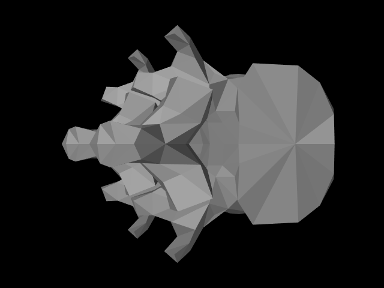
\includegraphics[]{images/LumbarFrameSpringNoflip}
\else
 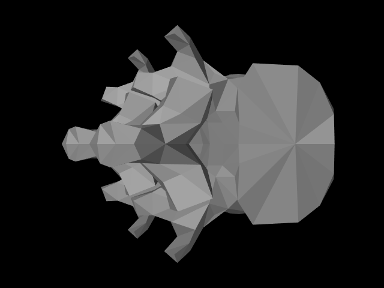
\includegraphics[width=3.75in]{images/LumbarFrameSpringNoflip}
\fi
\end{center}
\caption{LumbarFrameSpring model as it would appear if not rotated
about the x axis.}
\label{LumbarFrameSpringNoflip:fig}
\end{figure}

At this point in the construction, if the model were to be loaded, it
would appear as in Figure \ref{LumbarFrameSpringNoflip:fig}. To
correct the viewpoint, we rotate the entire model about the x axis
(line 29).  This is done using
\javamethodAlt{artisynth.core.mechmodels.MechModel.transformGeometry()}
{transformGeometry(X)}, which transforms the geometry of an entire
model using a rigid or affine transform.

The frame spring is created and added at lines 33-38, using the
methods described in Section \ref{CreatingFrameSprings:sec}, with
frame D set to the (initial) pose of {\tt lumbar1}.

Render properties are set starting at line 41. By default, a frame
spring renders as a pair of red, green, blue coordinate axes showing
frames C and D, along with a line connecting them. The line width and
the color of the connecting line are controlled by the line render
properties {\tt lineWidth} and {\tt lineColor}, while the length of
the coordinate axes is controlled by the special frame spring property
{\tt axisLength}.

To run this example in ArtiSynth, select {\sf All demos > tutorial >
LumbarFrameSpring} from the {\sf Models} menu. The model should load
and initially appear as in Figure \ref{LumbarFrameSpring:fig}.
Running the model (Section \ref{LoadingAndRunning:sec}) will cause
{\tt lumbar1} to fall slightly under gravity until the frame spring
arrests the motion. To get a sense of the spring's behavior, one can
interactively apply forces to {\tt lumbar1} using the pull manipulator
(see the section "Pull Manipulator" in the
\href{../uiguide/uiguide.html}{
ArtiSynth User Interface Guide}).

\subsection{Attachments}
\label{Attachments:sec}

ArtiSynth provides the ability to rigidly attach dynamic components to
other dynamic components, allowing different parts of a model to be
connected together.

\subsubsection{The attachment methods}

Attachments are made by adding to a {\tt MechModel} special {\it
attachment} components that manage the attachment physics as described
briefly in Section
\ref{PhysicsSimulation:sec}. At present, attachments
are implemented only for point-based components.  Modeling
applications do not generally handle the attachment components
directly, but instead use the followng {\tt MechModel} methods,
%
\begin{lstlisting}
  attachPoint (Point p1, Particle p2);
  attachPoint (Point p1, RigidBody body, Point3d loc);
  attachPoint (Point p1, RigidBody body);
  attachPoint (Point p1, FemElement3d elem);
  detachPoint (Point p1);
\end{lstlisting}
%
which attach a point {\tt p1} to either a particle, rigid body, or a
finite element.
\javamethodAlt{artisynth.core.mechmodels.MechModel.attachPoint(Point,RigidBody,Point3d)}
{attachPoint(p1, body, loc)} attaches {\tt p1} to {\tt body} at the
point {\tt loc} specified in body coordinates, while
\javamethodAlt{artisynth.core.mechmodels.MechModel.attachPoint(Point,RigidBody)}{attachPoint(p1,
body)} computes the attachment location based on the current position
and pose of {\tt p1} and {\tt body}.  Once {\tt p1} is attached, it
will in the {\it attached} state, as described in Section
\ref{DynamicVsParametric:sec}.
An attachment can be removed by calling 
\javamethod*[artisynth.core.mechmodels.MechModel]{detachPoint()}.
Finite element attachments are
discussed in Section \ref{NodeAttachments:sec}.

\subsubsection{Example: model with particle attachments}

\begin{figure}[h]
\begin{center}
\iflatexml
 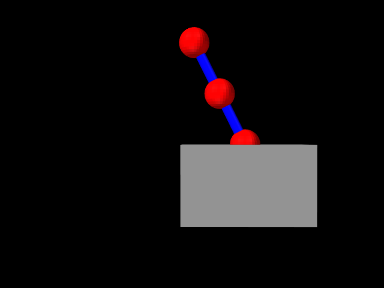
\includegraphics[]{images/ParticleAttachment}
\else
 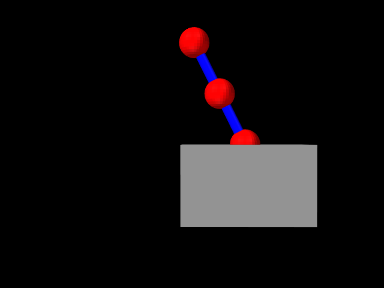
\includegraphics[width=3.75in]{images/ParticleAttachment}
\fi
\end{center}
\caption{ParticleAttachment model loaded into ArtiSynth.}
\label{ParticleAttachment:fig}
\end{figure}

A model illustrating particle-particle and particle-rigid body attachments
is defined in
%
\begin{verbatim}
  artisynth.demos.tutorial.ParticleAttachment
\end{verbatim}
%
and most of the code is shown here:
%
\lstset{numbers=left}
\begin{lstlisting}
   public Particle addParticle (MechModel mech, double x, double y, double z) {
      // create a particle at x, y, z and add it to mech
      Particle p = new Particle (/*name=*/null, /*mass=*/.1, x, y, z);
      mech.addParticle (p);
      return p;
   }

   public AxialSpring addSpring (MechModel mech, Particle p1, Particle p2){
      // create a spring connecting p1 and p2 and add it to mech
      AxialSpring spr = new AxialSpring (/*name=*/null, /*restLength=*/0);
      spr.setMaterial (new LinearAxialMaterial (/*k=*/20, /*d=*/10));
      spr.setPoints (p1, p2);
      mech.addAxialSpring (spr);
      return spr;
   }

   public void build (String[] args) {

      // create MechModel and add to RootModel
      MechModel mech = new MechModel ("mech");
      addModel (mech);

      // create the components
      Particle p1 = addParticle (mech, 0, 0, 0.55);
      Particle p2 = addParticle (mech, 0.1, 0, 0.35);
      Particle p3 = addParticle (mech, 0.1, 0, 0.35);
      Particle p4 = addParticle (mech, 0, 0, 0.15);
      addSpring (mech, p1, p2);
      addSpring (mech, p3, p4);
      // create box and set it's pose (position/orientation):
      RigidBody box =
         RigidBody.createBox ("box", /*wx,wy,wz=*/0.5, 0.3, 0.3, /*density=*/20);
      box.setPose (new RigidTransform3d (/*x,y,z=*/0.2, 0, 0));
      mech.addRigidBody (box);

      p1.setDynamic (false);               // first particle set to be fixed

      // set up the attachments
      mech.attachPoint (p2, p3);
      mech.attachPoint (p4, box, new Point3d (0, 0, 0.15));

      // increase model bounding box for the viewer
      mech.setBounds (/*min=*/-0.5, 0, -0.5, /*max=*/0.5, 0, 0);  
      // set render properties for the components
      setPointRenderProps (mech);
      setLineRenderProps (mech);
   }
%
\end{lstlisting}
\lstset{numbers=none}

The code is very similar to {\tt ParticleSpring} and {\tt
RigidBodySpring} described in Sections \ref{ParticleSpringExample:sec}
and \ref{RigidBodySpringExample:sec}, except that two convenience
methods, {\tt addParticle()} and {\tt addSpring()} are defined at
lines 1-15 to create particles and spring and add them to a {\tt
MechModel}. These are used in the {\tt build()} method to create four
particles and two springs (lines 24-29), along with a rigid body box
(lines 31-34). As with the other examples, particle {\tt p1} is set to
be non-dynamic (line 36) in order to fix it in place and provide a
ground.

The attachments are added at lines 39-40, with {\tt p2} attached to
{\tt p3} and {\tt p4} connected to the box at the location $(0, 0,
0.15)$ in box coordinates. 

Finally, render properties are set starting at line 43. In this
example, point and line render properties are set for the entire {\tt
MechModel} instead of individual components.  Since render properties
are inherited, this will implicitly set the specified render
properties in all sub-components for which these properties are not
explicitly set, either locally or in an intermediate ancestor.

To run this example in ArtiSynth, select {\sf All demos > tutorial >
ParticleAttachment} from the {\sf Models} menu. The model should load
and initially appear as in Figure \ref{ParticleAttachment:fig}.
Running the model (Section \ref{LoadingAndRunning:sec}) will cause the
box to fall and swing under gravity.

\subsection{Simulation control properties}

Both \javaclass[artisynth.core.workspace]{RootModel} and
\javaclass[artisynth.core.mechmodels]{MechModel} contain properties
that control the simulation behavior. One of the most important of
these is {\tt maxStepSize}. By default, simulation proceeds using the
{\tt maxStepSize} value defined for the root model. A {\tt MechModel}
contained within the root model may also request a smaller step size
by specifying a smaller value for its own {\tt maxStepSize} property.
For all models, the maximum step size may be set and queried
using
%
\begin{lstlisting}
  void setMaxStepSize (double maxh);
  double getMaxStepSize();
\end{lstlisting}
%

Another important simulation property is {\tt integrator} in {\tt
MechModel}, which determines the type of integrator used for the
physics simulation. The property value is the enumerated type
{\tt MechSystemSolver.Integrator}, and it can currently
be set to the following values:

\begin{description}

\item[ForwardEuler]\mbox{}

First order forward Euler integrator. Unstable for stiff systems.

\item[SymplecticEuler]\mbox{}

First order symplectic Euler integrator, more energy conserving
that forward Euler. Unstable for stiff systems.

\item[RungeKutta4]\mbox{}

Fourth order Runge Kutta integrator, quite accurate but also unstable
for stiff systems.

\item[ConstrainedBackwardEuler]\mbox{}

First order backward order integrator. Generally stable for stiff systems.

\item[Trapezoidal]\mbox{}

Second order trapezoidal integrator. Generally stable for stiff
systems, but slightly less so than {\tt ConstrainedBackwardEuler}.

\end{description}

The term "Unstable for stiff systems" means that the integrator is
likely to go unstable in the presence of "stiff" systems, which
typically include systems containing finite element models.  The
default value for {\tt integrator} is {\tt ConstrainedBackwardEuler}.

Another {\tt MechModel} simulation property is {\tt stabilization},
which controls the stabilization method used correct drift from
position constraints and correct interpenetrations due to collisions.
The property value is the enumerated type {\tt
MechSystemSolver.PosStabilization}, and it has two values:

\begin{description}

\item[GlobalMass]\mbox{}

Uses only a diagonal mass matrix for the MLCP that is solved to
determine the position corrections. This is default method.

\item[GlobalStiffness]\mbox{}

Uses a stiffness-corrected mass matrix for the MLCP that is solved to
determine the position corrections. Slower than {\tt GlobalMass}, but
more likely to produce stable results, particularly for
problems involving FEM collisions.

\end{description}

